\section{Experiments}
We empirically evaluate a few matching algorithms in different settings of utility and excitement initialization, and identify algorithms that can produce matches with high stability, high social welfare and high consistency.
\subsection{Experimental Set-up}
% 0.5-1 page
% \begin{itemize}
%     \item Algorithms we are evaluating
%     \begin{itemize}
%         \item MPDA, WPDA
%         \item Probabilistic-based that always selects the best stable matching with a probability
%         \item Probabilistic-based that always selects the best matching with a probability
%         \item [Stretch] Deterministic algorithm that always selects the best sw with a consistency above a certain threshold
%     \end{itemize}
%     \item Dynamics
%     \item Number of agents, time steps, etc.
%     \item Evaluation set-up
% \end{itemize}
\paragraph{Dynamics Setting} For each agent, we independently initialize each utility value by sampling from a normal distribution $\mathcal{N}(\mu_u, \sigma_u^2)$ with scalar mean $\mu_u \in \mathbb{R}$ and variance $\sigma_u^2 \in \mathbb{R}$. For each utility value $x$, we clip it at 0 with $x \leftarrow \max(x, 0)$ to ensure it is non-negative. We further normalize the utilities such that each agent's utility vector has a total sum of 1. In addition, we set each agent's excitement values by again independently sampling from a normal distribution $\mathcal{N}(\mu_e, \sigma_e^2)$. We clip each excitement value at 0 to ensure that the excitement is non-negative.

\paragraph{Algorithms} We implement both the Men Proposing Deferred Acceptance (MPDA) and the Women Proposing Deferred Acceptance (WPDA) algorithms~\cite{galeshapley1962}, which are guaranteed to return a stable matching. In addition, we implement a family of deterministic algorithms (Det) and a family of probabilistic algorithms (Prob), described as follows.

\textit{\textbf{Det}}: This is a family of algorithms parameterized by $c \in [0, 1]$ and returns a perfect matching satisfying $$M^{t+1} = \argmax_{\mbox{consistency}(M^t, M) \ge c}{\mbox{sw}(M)}.$$
% In other words, the generated matching $M^{t+1}$ is the matching maximizing the social welfare subjected to the condition that the consistency is at least $c$ compared to the most recent match.
For computational efficiency, we approximate this algorithm by first fixing $N * c$ couples in $M^t$ that have the highest social welfare according to the updated utilities $\overrightarrow{u}^{t+1}, \overrightarrow{v}^{t+1}$, and then perform the Hungarian Algorithm~\cite{Kuhn55thehungarian,Kuhn56thehungarian,Munkres1957Assignment} over the remaining men and women to obtain the maximum weight perfect bipartite matching, where the weight between a man node $m_i$ and a woman node $w_j$ is $u_i^{t+1}(w_j) + v_j^{t+1}(m_i)$. As a result, the generated new matching has at least consistency $c$ and a reasonably large social welfare.

\textit{\textbf{Prob}}: This family of algorithms is parameterized by a probability value $p$ and finds a matching as follows:
$$M^{t+1} = \begin{cases} \argmax_M{\mbox{sw}(M)} &\text{with probability $1-p$}\\ M^t &\text{with probability $p$}\end{cases}.$$
As a result, the expected consistency is at least $p$. We find $\argmax_M{\mbox{sw}(M)}$ by running the Hungarian algorithm on the full bipartite graph.

\textit{\textbf{Prob-Stable}} A variant of the probabilistic algorithm is to always return a maximum social welfare \textit{stable} matching $\argmax_{\text{stable $M$}}{\mbox{sw}(M)}$ with probability $1-p$. However, in the case where we keep the previous matching $M^t$, since $M^t$ might not be stable with the updated utilities, Prob-Stable is not guaranteed to have stable matches all the time.


\subsection{Results}
\begin{figure}
    \centering
    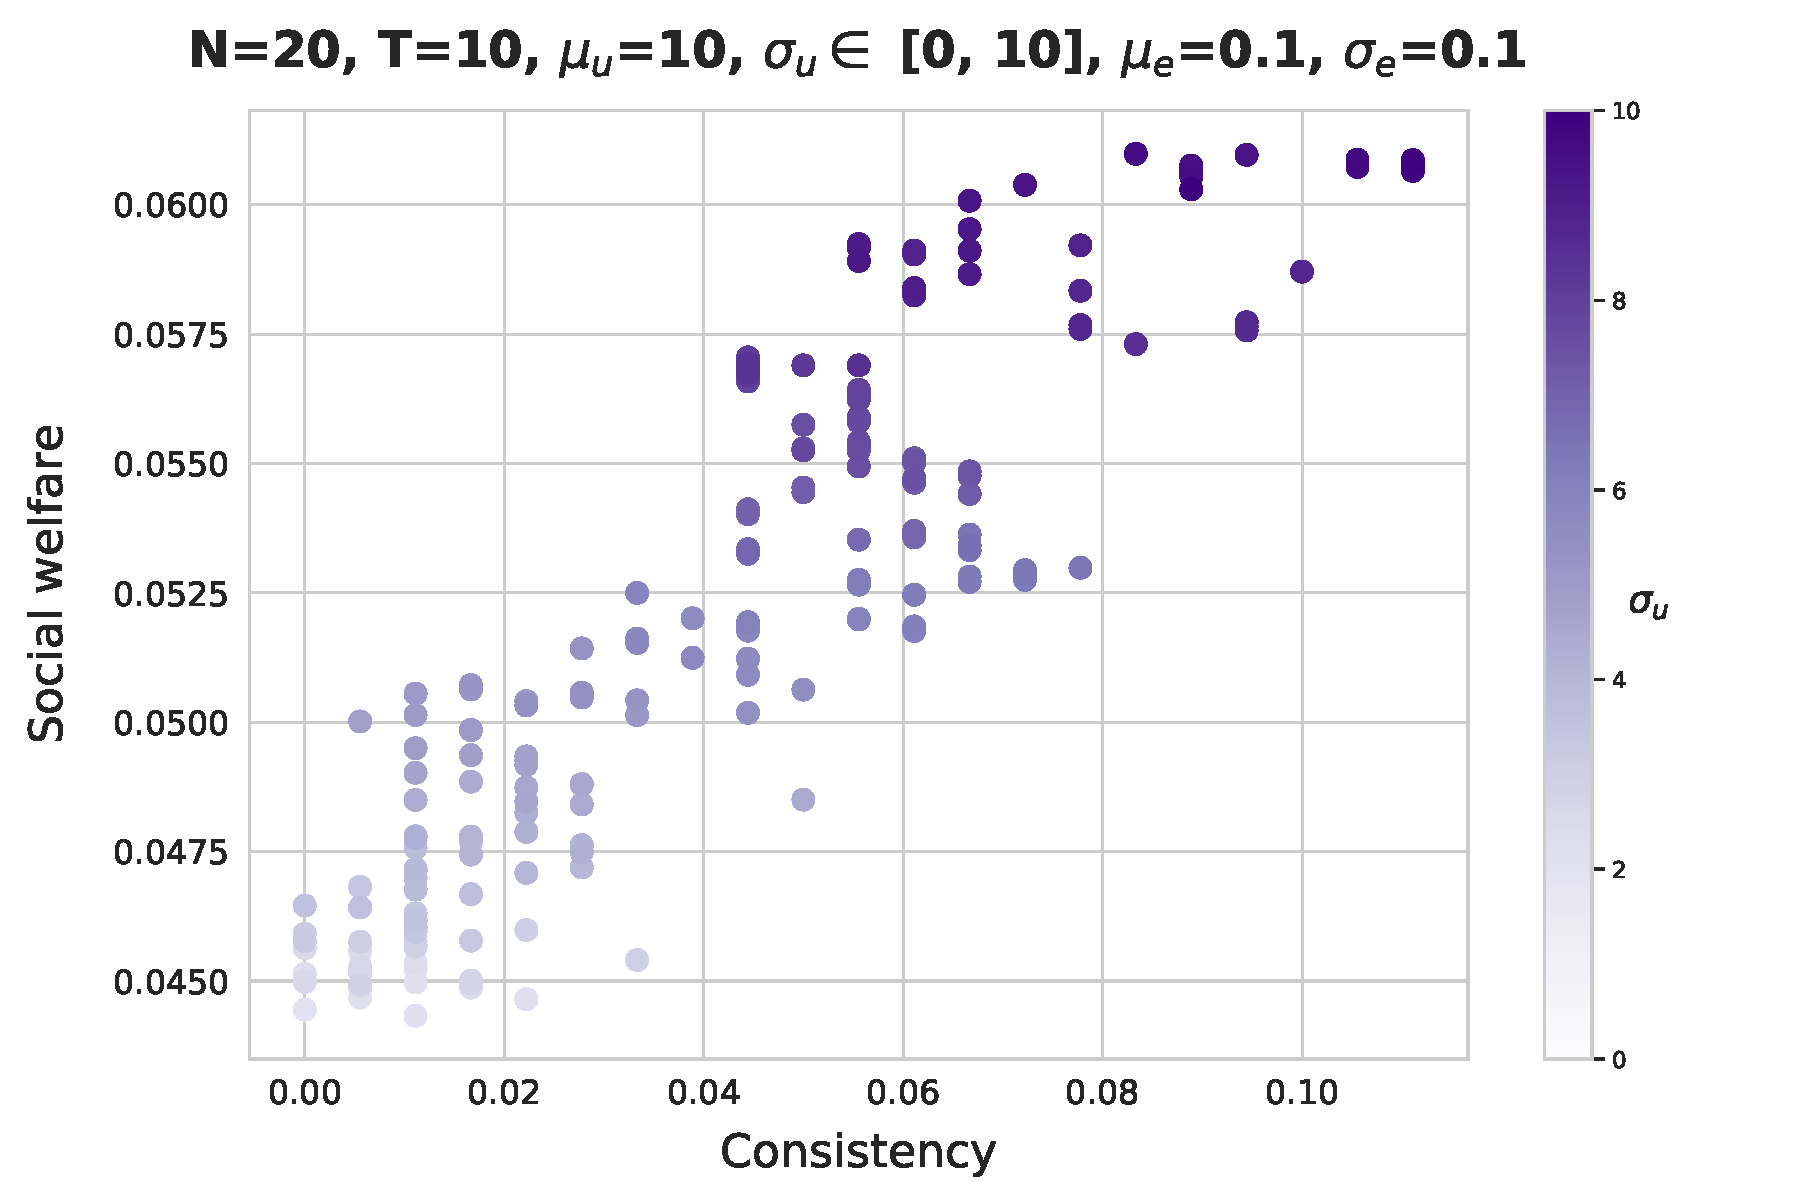
\includegraphics[width=0.32\linewidth]{figures/mpda_dynamics_initliazation.pdf}
    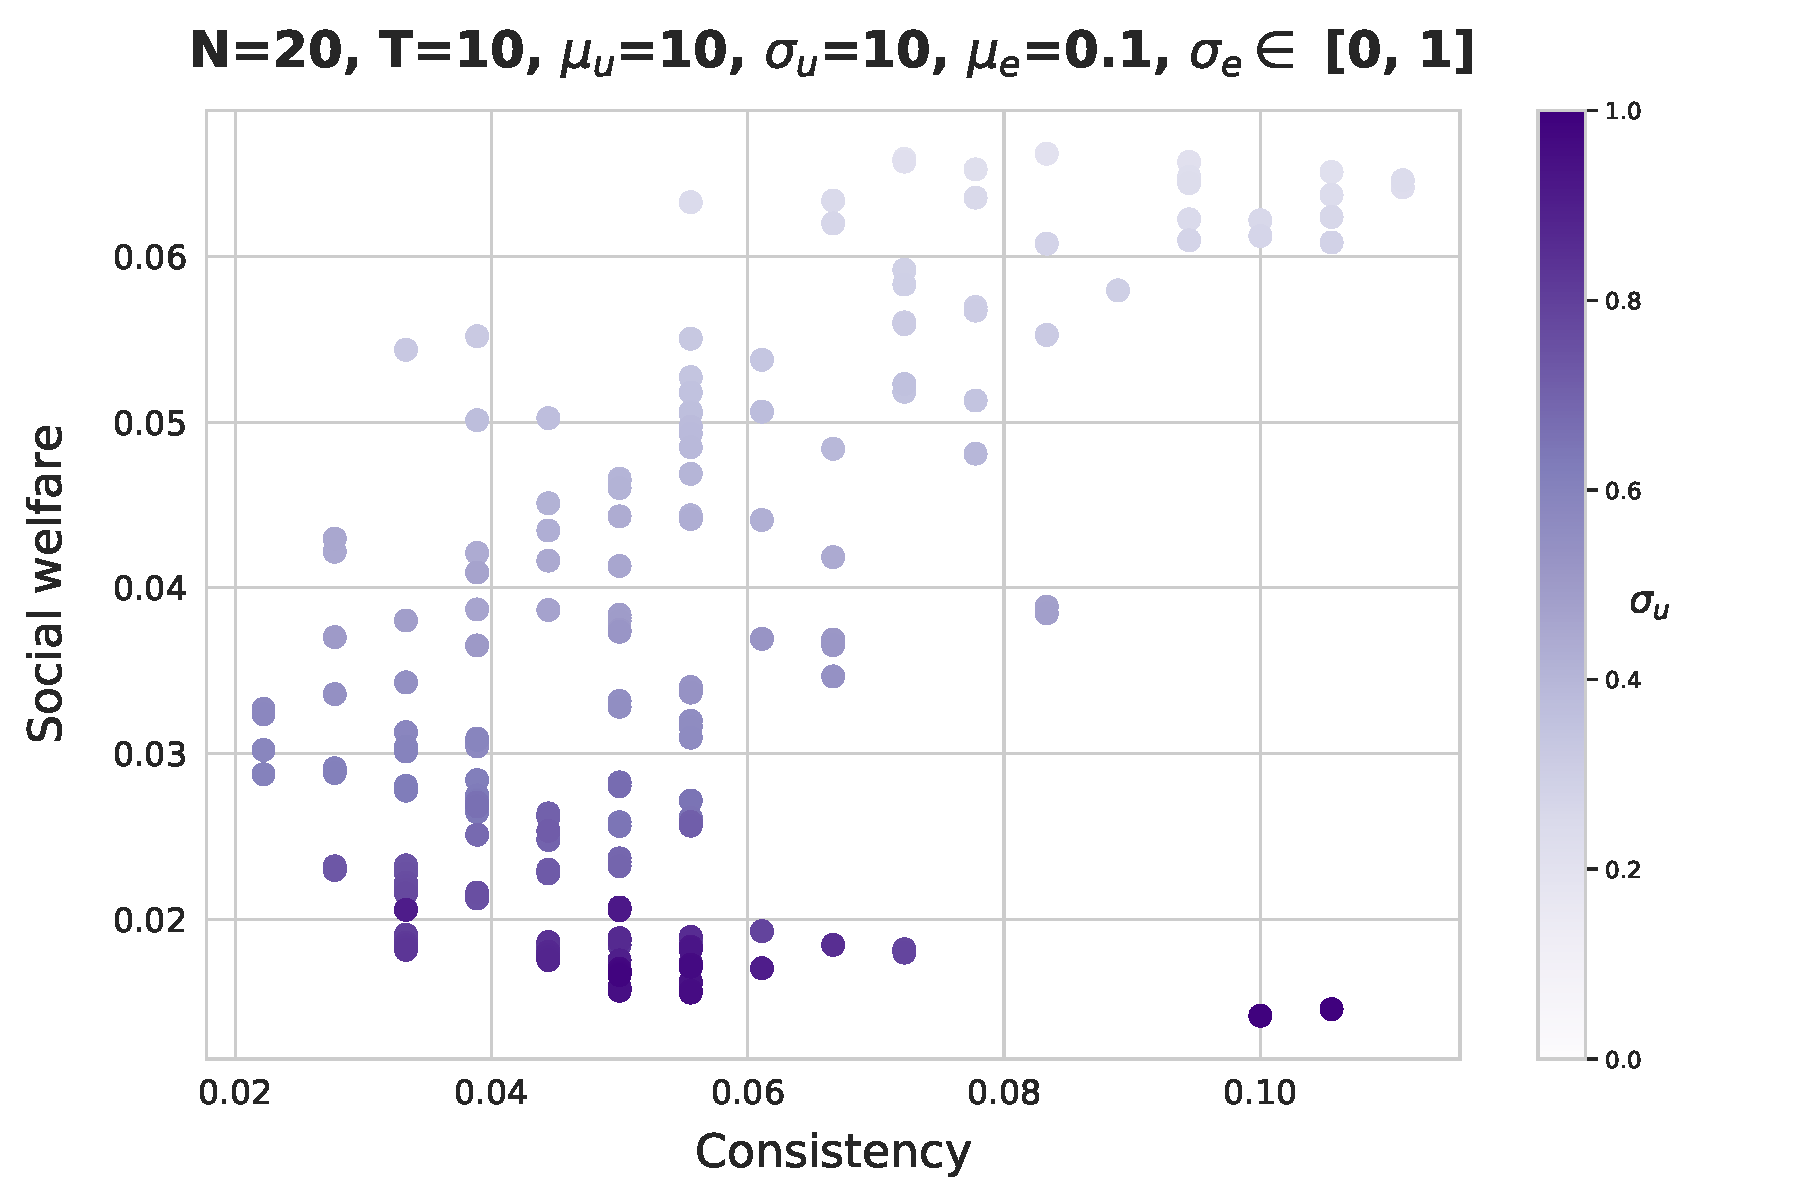
\includegraphics[width=0.32\linewidth]{figures/mpda_dynamics_excitement_std.pdf}
    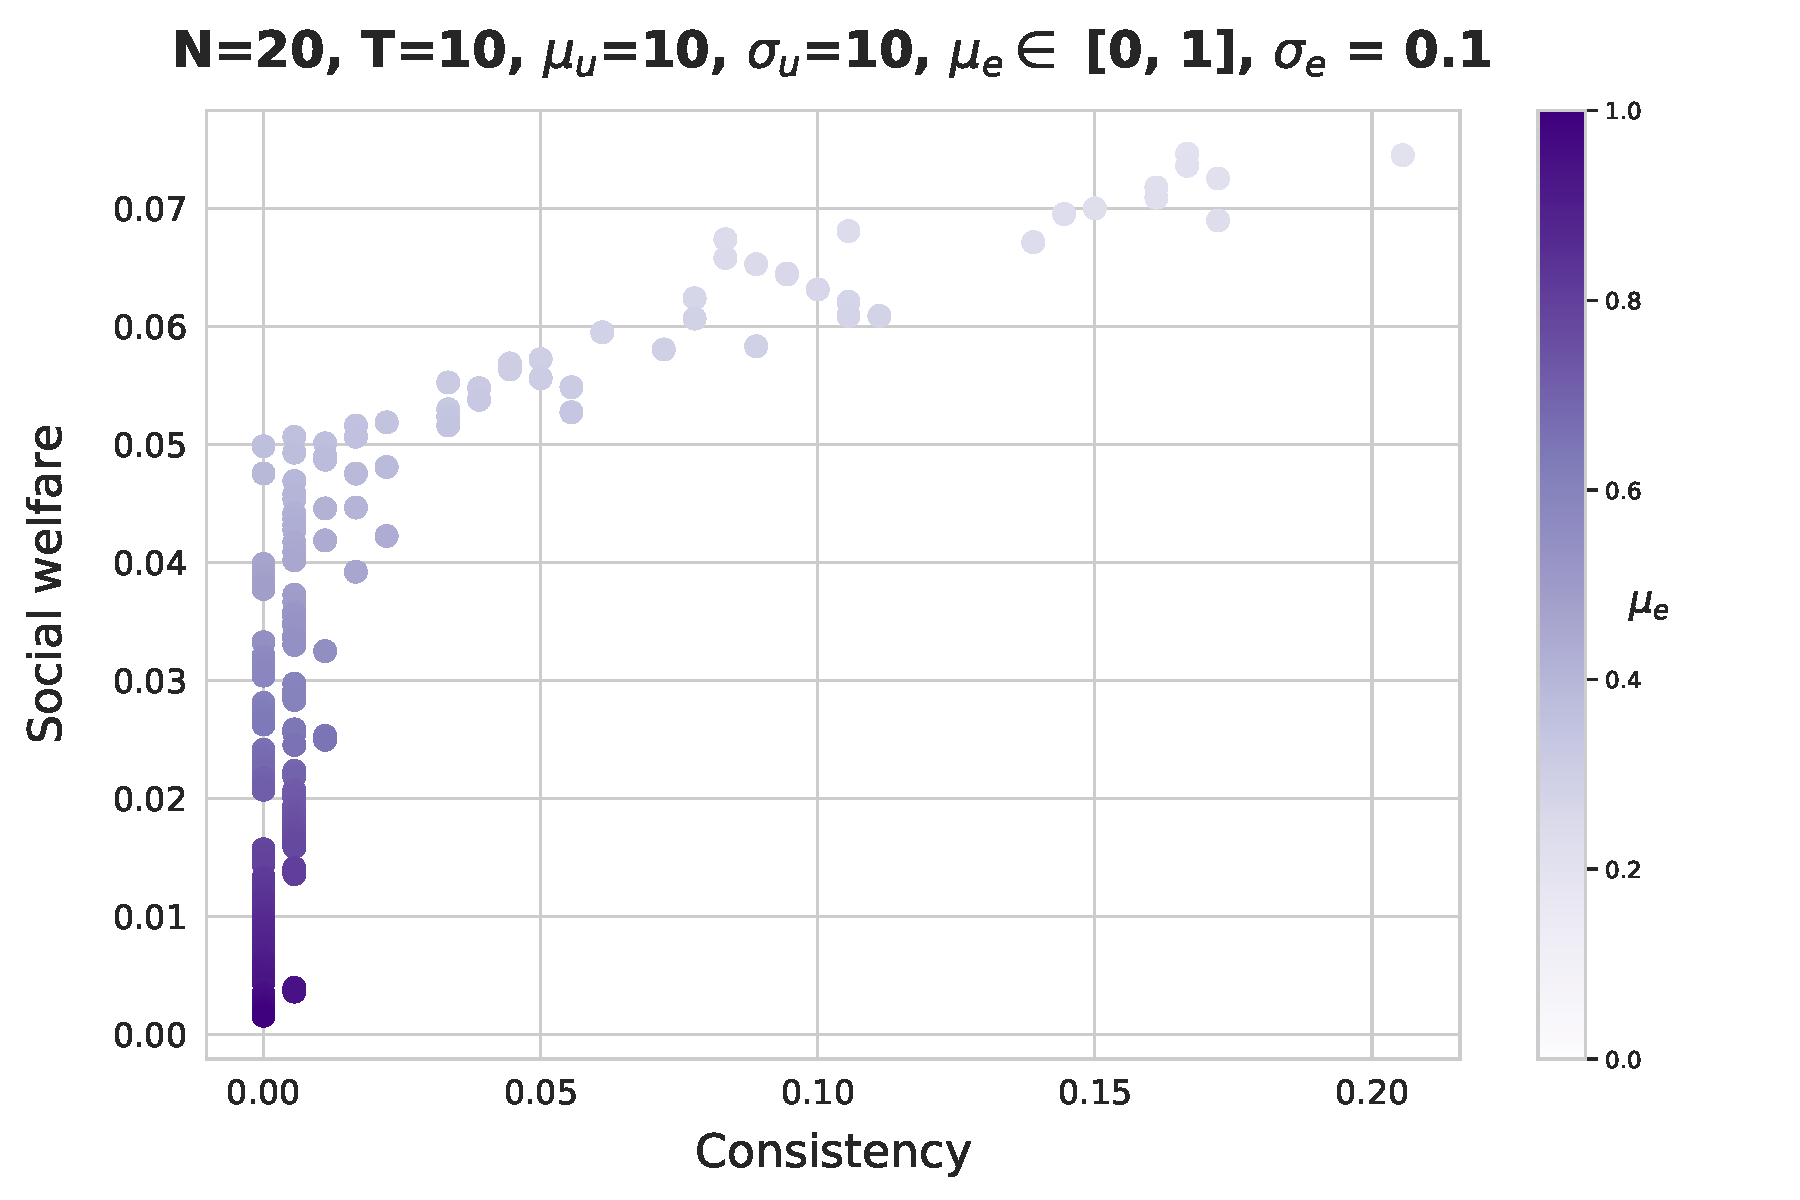
\includegraphics[width=0.32\linewidth]{figures/mpda_dynamics_excitement_mean.pdf}
     \caption{Mean social welfare vs. consistency for MPDA applied in various settings with 20 men/women and 10 time steps. (Left) Fixed excitement with varying utilities initialization (fixed mean). (Middle) Fixed utilities initialization but varying excitement (fixed mean) (b) fixed initialization varying excitement (fixed mean). (Right) Fixed utilities initialization but varying excitement (fixed variance).}
    \label{fig:mpda_dynamics}
\end{figure}
% \begin{figure}
%     \centering
%         \begin{subfigure}[b]{0.49\textwidth}
%          \centering
%          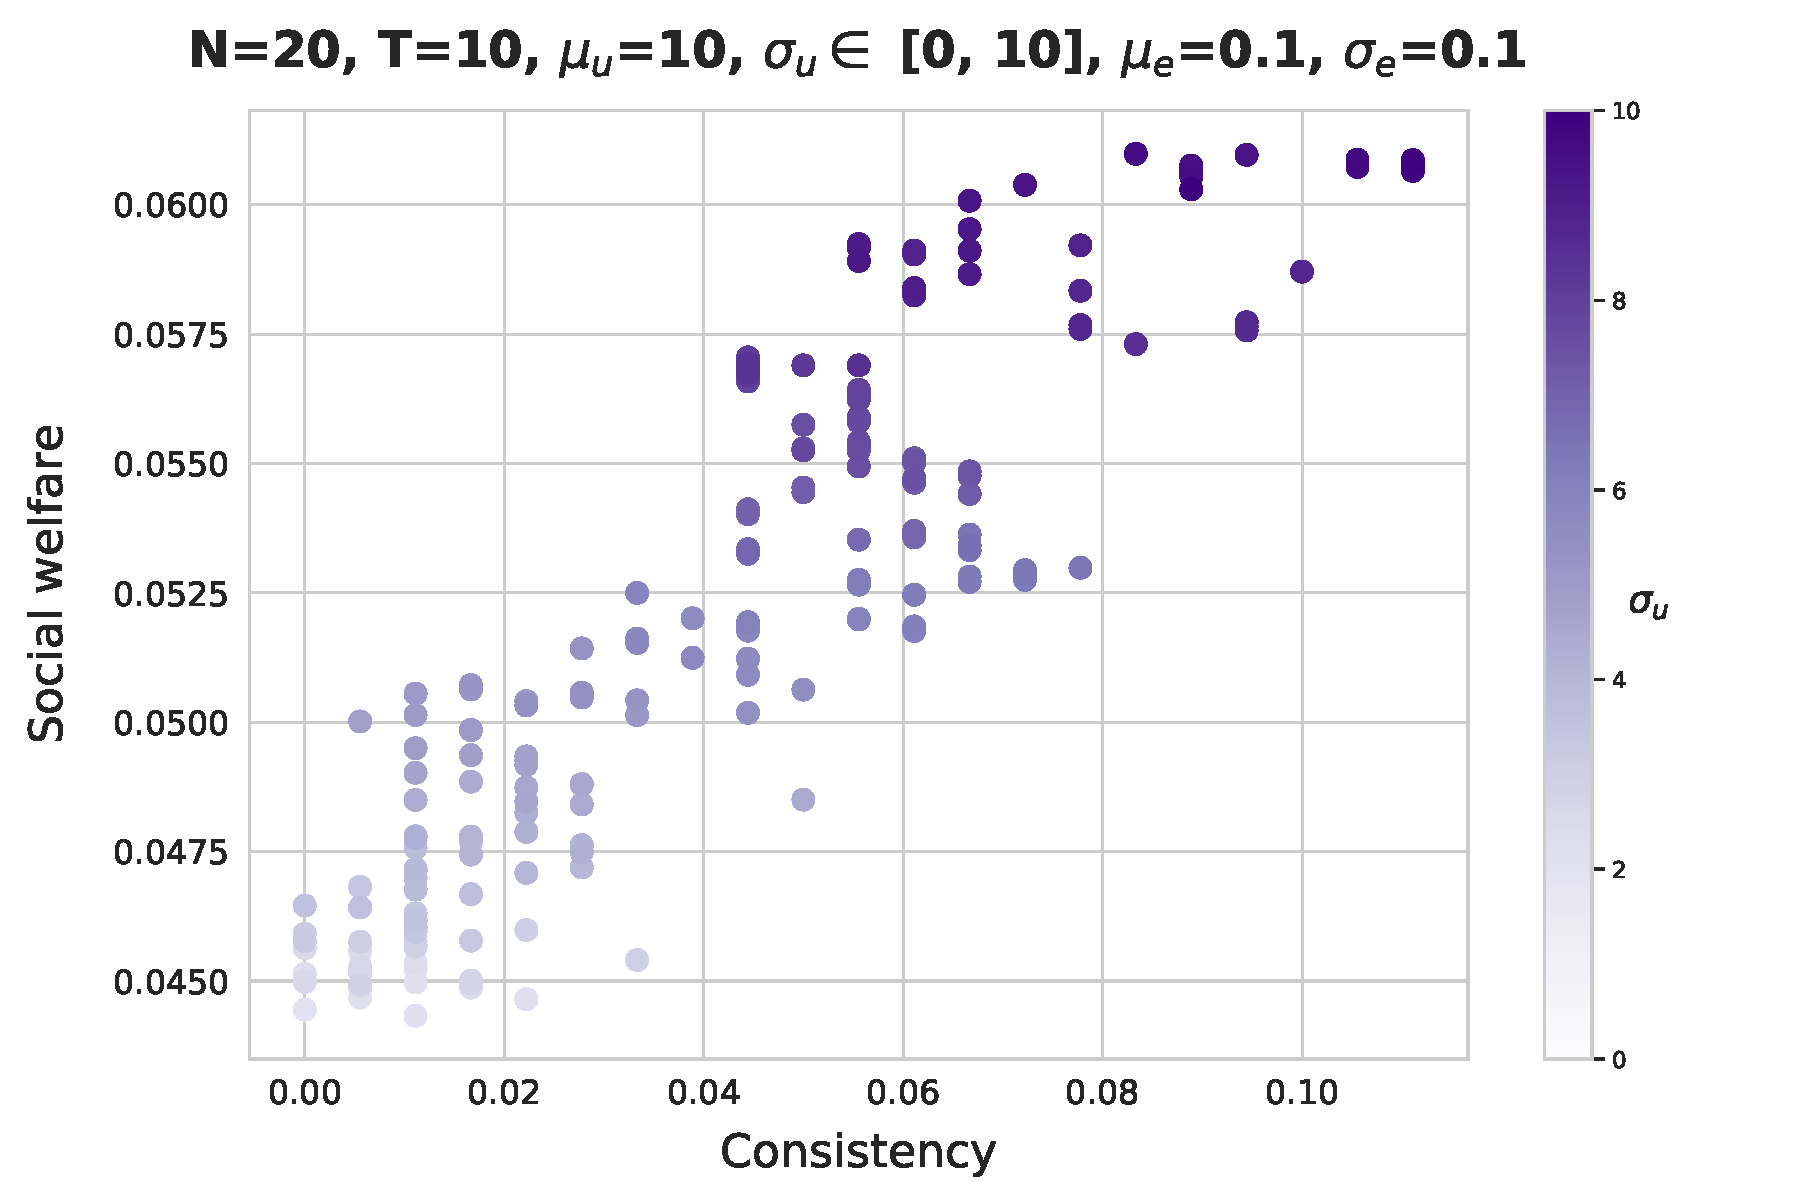
\includegraphics[width=\textwidth]{figures/mpda_dynamics_initliazation.pdf}
%          \caption{Dynamic Initialization}
%          \label{fig:init}
%         \end{subfigure}
%          \begin{subfigure}[b]{0.49\textwidth}
%          \centering
%          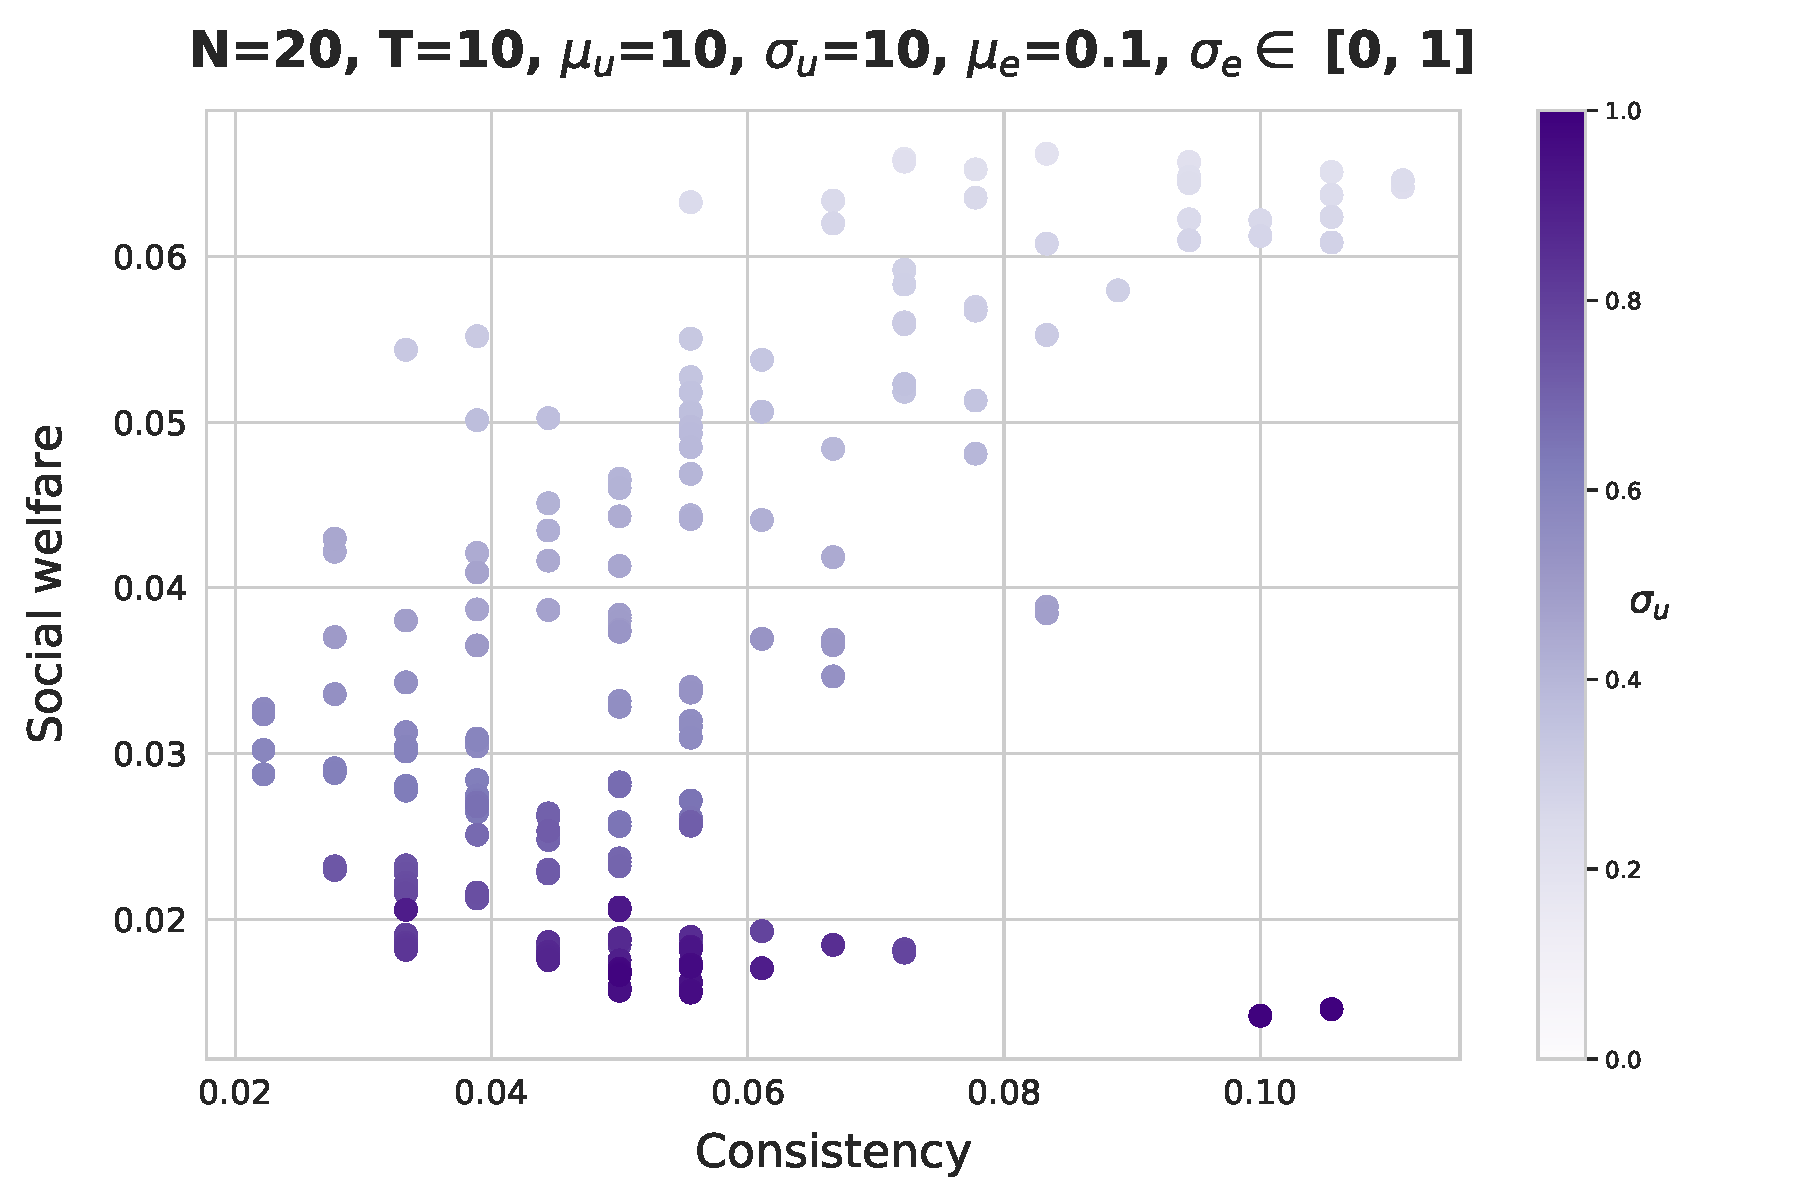
\includegraphics[width=\textwidth]{figures/mpda_dynamics_excitement_std.pdf}
%          \caption{Dynamic Excitement}
%          \label{fig:excite_std}
%      \end{subfigure}
%          \begin{subfigure}[b]{0.49\textwidth}
%          \centering
%          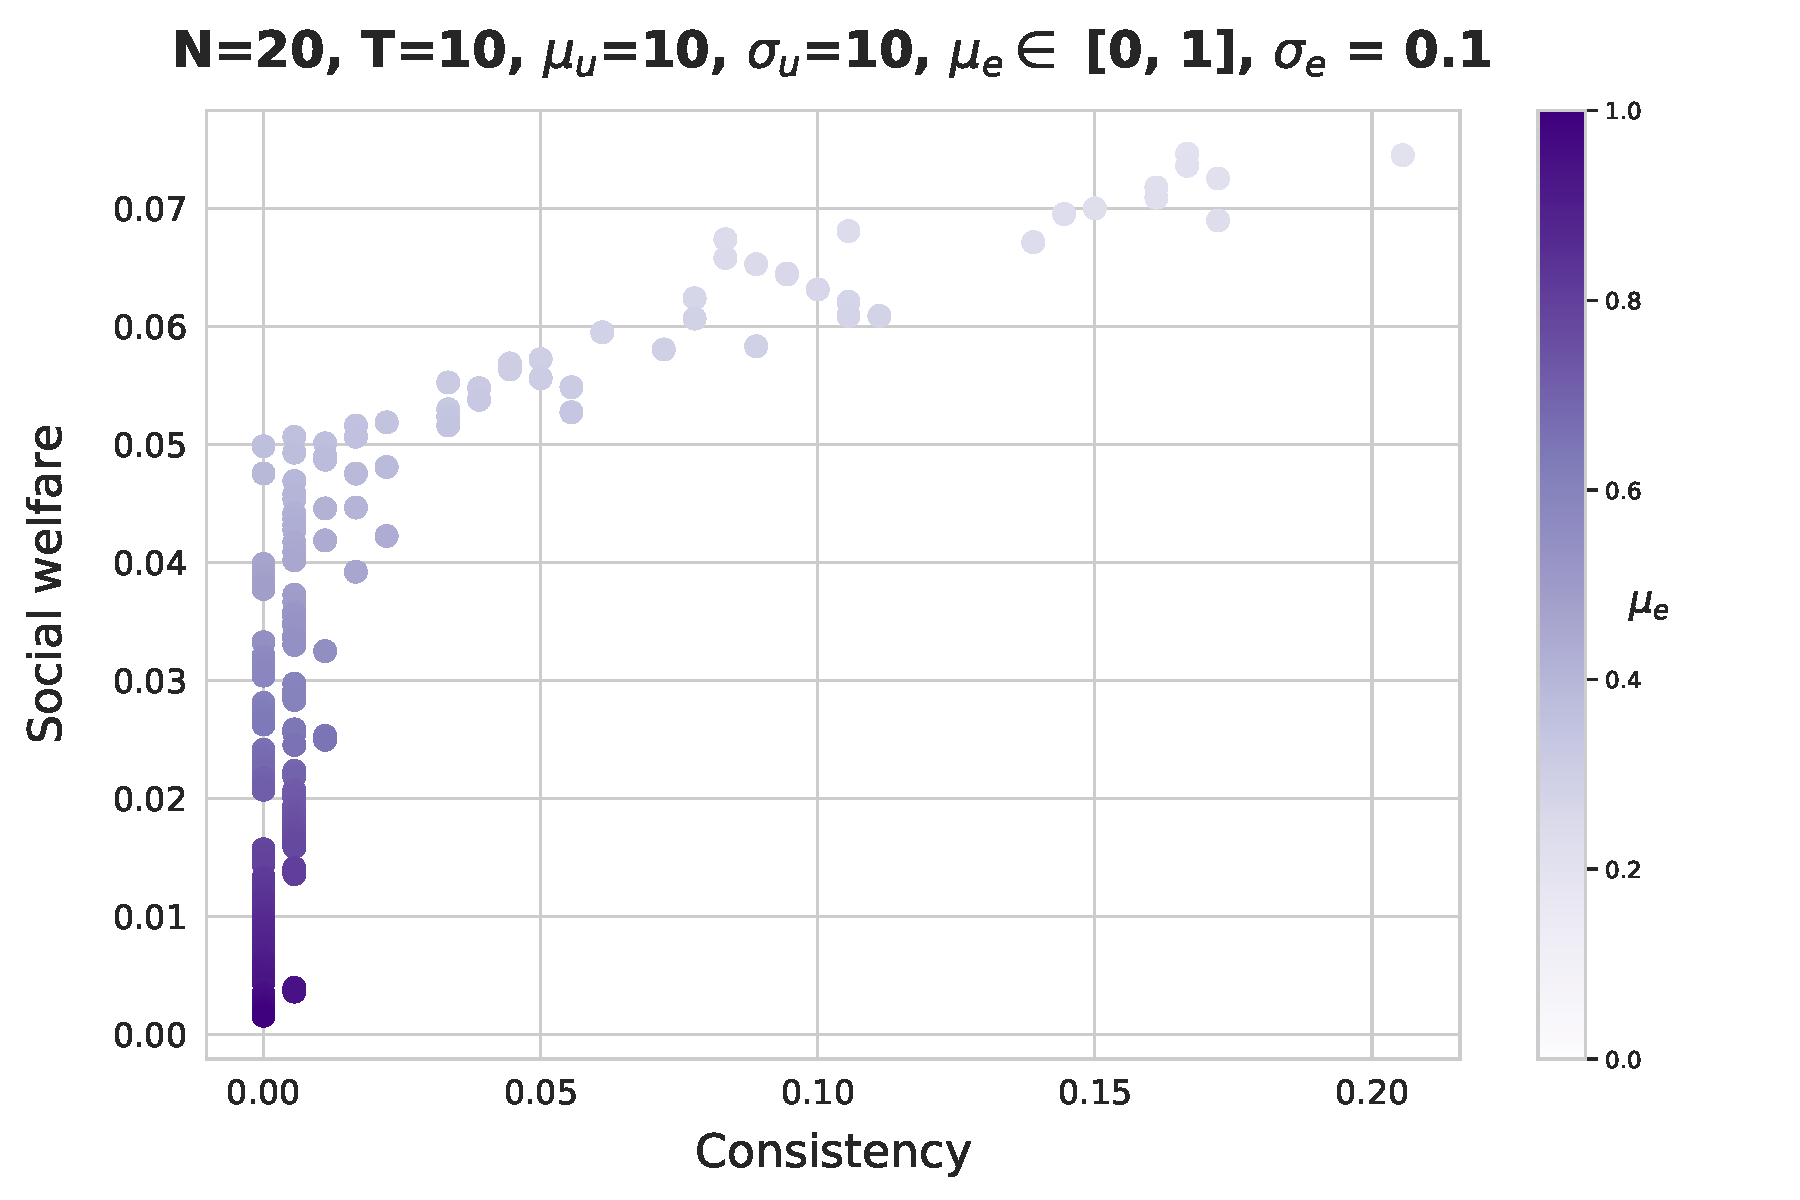
\includegraphics[width=\textwidth]{figures/mpda_dynamics_excitement_mean.pdf}
%          \caption{Dynamic Excitement}
%          \label{fig:excite_mean}
%      \end{subfigure}
%      \caption{Mean social welfare vs. consistency for MPDA applied to two dyanmic scenarios; (a) fixed excitement; (b) fixed initialization varying excitement (fixed mean); (c) fized initialization with varying excitement (fixed standard deviation).}
%     \label{fig:mpda_dynamics}
% \end{figure}

\paragraph{Dynamics}

\paragraph{Algorithms} We run MPDA, WPDA, Det, Prob and Prob-Stable 

\paragraph{Stability Social Welfare}
% 0.5 - 1 page
% Figures and analysis
% \begin{itemize}
%     \item Evaluation of the algorithms (trade-off plot)
%     \begin{itemize}
%         \item scatter plot for the algorithm family
%         \item variance plot for the algorithm family
%     \end{itemize}
%     \item Evaluation with various dynamics
%     \begin{itemize}
%         \item Plot the trade off curve with MPDA and update with match
%     \end{itemize}
% \end{itemize}
